%
% FH Technikum Wien
% !TEX encoding = UTF-8 Unicode
%
% Erstellung von Master- und Bachelorarbeiten an der FH Technikum Wien mit Hilfe von LaTeX und der Klasse TWBOOK
%
% Um ein eigenes Dokument zu erstellen, müssen Sie folgendes ergänzen:
% 1) Mit \documentclass[..] einstellen: Master- oder Bachelorarbeit, Studiengang und Sprache
% 2) Mit \newcommand{\FHTWCitationType}.. Zitierstandard festlegen (wird in der Regel vom Studiengang vorgegeben - bitte erfragen)
% 3) Deckblatt, Kurzfassung, etc. ausfüllen
% 4) und die Arbeit schreiben (die verwendeten Literaturquellen in Literatur.bib eintragen)
%
% Getestet mit TeXstudio mit Zeichenkodierung ISO-8859-1 (=ansinew/latin1) und MikTex unter Windows
% Zu beachten ist, dass die Kodierung der Datei mit der Kodierung des paketes inputenc zusammen passt!
% Die Kodierung der Datei twbook.cls MUSS ANSI betragen!
% Bei der Verwendung von UTF8 muss dnicht nur die Kodierung des Dokuments auf UTF8 gestellt sein, sondern auch die des BibTex-Files!

\documentclass[MGS,Master,english]{twbook}%\documentclass[Bachelor,BMR,german]{twbook}
\usepackage[utf8]{inputenc}
\usepackage[T1]{fontenc}
\usepackage{cite}
\usepackage[numbers]{natbib}
\usepackage{booktabs}
\usepackage{wrapfig}

%
% Bitte in der folgenden Zeile den Zitierstandard festlegen
\newcommand{\FHTWCitationType}{IEEE} % IEEE oder HARVARD möglich - wenn Sie zwischen IEEE und HARVARD wechseln, bitte die temorären Dateien (aux, bbl, ...) löschen
%
\ifthenelse{\equal{\FHTWCitationType}{HARVARD}}{\usepackage{harvard}}{\usepackage{bibgerm}}

% Definition Code-Listings Formatierung:
\usepackage[final]{listings}
\lstset{captionpos=b, numberbychapter=false,caption=\lstname,frame=single, numbers=left, stepnumber=1, numbersep=2pt, xleftmargin=15pt, framexleftmargin=15pt, numberstyle=\tiny, tabsize=3, columns=fixed, basicstyle={\fontfamily{pcr}\selectfont\footnotesize}, keywordstyle=\bfseries, commentstyle={\color[gray]{0.33}\itshape}, stringstyle=\color[gray]{0.25}, breaklines, breakatwhitespace, breakautoindent}
\lstloadlanguages{[ANSI]C, C++, [gnu]make, gnuplot, Matlab}

%Formatieren des Quellcodeverzeichnisses
\makeatletter
% Setzen der Bezeichnungen für das Quellcodeverzeichnis/Abkürzungsverzeichnis in Abhängigkeit von der eingestellten Sprache
\providecommand\listacroname{}
\@ifclasswith{twbook}{english}
{%
    \renewcommand\lstlistingname{Code}
    \renewcommand\lstlistlistingname{List of Code}
    \renewcommand\listacroname{List of Abbreviations}
}{%
    \renewcommand\lstlistingname{Quellcode}
    \renewcommand\lstlistlistingname{Quellcodeverzeichnis}
    \renewcommand\listacroname{Abkürzungsverzeichnis}
}
% Wenn die Option listof=entryprefix gewählt wurde, Definition des Entyprefixes für das Quellcodeverzeichnis. Definition des Macros listoflolentryname analog zu listoflofentryname und listoflotentryname der KOMA-Klasse
\@ifclasswith{scrbook}{listof=entryprefix}
{%
    \newcommand\listoflolentryname\lstlistingname
}{%
}
\makeatother
\newcommand{\listofcode}{\phantomsection\lstlistoflistings}

% Die nachfolgenden Pakete stellen sonst nicht benötigte Features zur Verfügung
\usepackage{blindtext}

%
% Einträge für Deckblatt, Kurzfassung, etc.
%
\title{%
	Using LLVM/Clang to to maintain the abstraction level of Object Oriented Programming, yet abide SOA rules\\
	\large How compiler technology could possibly make a link between conflicting programming paradigms}
\author{Julian Müller, BSc.}
\studentnumber{1610585015}
%\author{Titel Vorname Name, Titel\and{}Titel Vorname Name, Titel}
%\studentnumber{XXXXXXXXXXXXXXX\and{}XXXXXXXXXXXXXXX}
\supervisor[Supervisor]{Stefan Reinalter, DI}
\secondsupervisor[Second Supervisor]{Prof. Alexander Hofmann, DI}

\place{Wien}

\outline{This work will prospect the possibility of using compiler technology as a mediator between the conflicting programming paradigms/philosophies \textit{OOP} and \textit{DoD}.\\While Object oriented programming is often praised for its benefits on abstraction and maintainability, it encourages programmers to design inefficient datalayouts. Specifically in game engineering, where performance is a constitutive factor for a product's success, data oriented solutions and influences are on the rise. While it is debated, wether or not performant data layouts inevitably entail challenging maintenance, surely the base concepts of \textit{objects} are well observable in a game. Therefore this will be an attempt to make object oriented programming a valid option for ever rising demands on performance.\\
To do so this thesis will investigate key concepts of both paradigms, as well as hardware specifics in modern computer architectures to explicate the reasons for their good/bad interaction with the hardware.\\
A prototypical implementation of a source-to-source transformation tool called \textit{COOP} (\textbf{C}ache friendly \textbf{O}bject \textbf{O}riented \textbf{P}rogramming), developed in Clang's LibTooling environment, will determine wether or not compiler technology can be used to achieve a performance optimization on a classically OOP abidant target code base.}
\keywords{Object Oriented Programming, OOP, Structure Of Arrays, SOA, Data Oriented Design, Compiler, LLVM, Clang}

\acknowledgements{TODO dankschee}

\begin{document}

%Festlegungen für den HARVARD-Zitierstandard
\ifthenelse{\equal{\FHTWCitationType}{HARVARD}}{
\bibliographystyle{Harvard_FHTW_MR}%Zitierstandard FH Technikum Wien, Studiengang Mechatronik/Robotik, Version 1.2e
\citationstyle{dcu}%Correct citation-style (Harvardand, ";" between citations, "," between author and year)
\citationmode{abbr}%use "et al." with first citation

%Englisch
\newcommand{\citepic}[1]{(Source: \protect\cite{#1})}%Zitat: Bild
\newcommand{\citefig}[2]{(Source: \protect\cite{#1}, p. #2)}%Zitat: Bild aus Dokument

\newcommand{\citefigm}[2]{(Source: taken with modification from \protect\cite{#1}, p. #2)}%Zitat: modifiziertes Bild aus Dokument
\newcommand{\citep}{\citeasnoun}%In-Line Zitiat entweder mit \citep{} oder \citeasnoun{}
\newcommand{\acessedthrough}{Available at:}%Für URL-Angabe
\newcommand{\acessedthroughp}{Available through:}%Für URL-Angabe (Geschützte Datenbank, Zugriff durch FH)
\newcommand{\acessedat}{Accessed}%Für URL-Datum-Angabe
\newcommand{\singlepage}{p.}%Für Seitenangabe (einzelne Seite)
\newcommand{\multiplepages}{pp.}%Für Seitenangabe (mehrere Seiten)
\newcommand{\chapternr}{Ch.}%Für Kapitelangabe
\renewcommand{\harvardand}{\&}%Harvardand in Zitaten
\newcommand{\abstractonly}{Abstract only}
\newcommand{\edition}{~edition}%Edition -> note, that you have to write "edition = {2nd},"!
}

%CUSTOM
\newcommand{\mc}[1]{\cite{#1}}
\newcommand{\mcp}[2]{\cite[p. #2]{#1}}
\newcommand{\mcpic}[1]{(Source: \mc{#1})}
\newcommand{\mcppic}[2]{(Source: \mcp{#1}{#2})}

\newcommand{\reffig}[1]{Fig. \ref{#1}}
\newcommand{\reffigp}[1]{(see \reffig{#1})}

\newcommand{\refcode}[1]{Code \ref{#1}}
\newcommand{\refcodep}[1]{(see \refcode{#1})}

\newcommand{\refsec}[1]{Section \ref{#1}}
\newcommand{\refsecp}[1]{(see \refsec{#1})}

\newcommand{\reftable}[1]{Table \ref{#1}}
\newcommand{\reftablep}[1]{(see \reftable{#1})}

\maketitle

%
% .. und hier beginnt die eigentliche Arbeit. Viel Erfolg beim Verfassen!
%
\chapter{Conflicting Paradigms}
Numerous programming paradigms exist for even more general programming languages. Each of them come with different perks and offer different perspectives for a problem. Different programming paradigms, however do not necessarily exclude each other. Languages like \textit{Scala} for example combine functional and object oriented programming.\\
This thesis will specifically concentrate on \textit{Object-Oriented Programming} (OOP) and \textit{Data-Oriented Design} (DoD). Whether or not data oriented design is even to be considered a programming paradigm is debatable \mcp{fabian}{1}. However its fundamental ideas (specifically concerning data layout) conflict with those of existing paradigms like OOP. Therefore to maintain consistency in this manner of comparison, it will be mentioned accordingly.\\ 
Depending on the domain, certain programmers will have different answers to the question which of both should be preferred. Each party will make compelling arguments to why their choice is mandatory. This is because those paradigms (partially) solve different problems and therefore offer dissenting perspectives on problems and their respective solutions for them.
To understand why \textit{Object Oriented Programming} and \textit{Data Oriented Design} are rather cannibalistic to each other, it is important to first have a look at what they are trying to solve, independently.

\section{Object Oriented Programming / AOS}\label{OOP}
Starting with punch cards, each iteration of new programming generations provided new forms of abstraction for programmers, be it control flow statements, type systems, data structures like native arrays. When machine code started to simplify operations, FORTRAN partly introduced portability as early as 1957; LISP introduced symbolic processing and automated memory management until finally Simula/67 introduced objects in the 1960s \mc{louden}\mc{hopl}.
Object Oriented Programming could not be called popular until the 1970s or 1980s, when Stroustrup created C++. Originally OOP was meant to be the way to go for creating graphics based applications  \mc{about_oop}. This makes sense, since tree like data structures (e.g. GUIs) containing entities with shared behavior can easily be described with polymorphism.\\
OOP shines, whenever the problem to be modeled can be abstracted to one or more base classes, that define shared state and/or behavior. Even though some languages allow for a subclass to "\textit{exclude variables and/or methods which would otherwise have been inherited from the superclass(es)}" \mcp{what_is_oop}{4} the general concept of objects usually includes derivation and extending base behavior.\\
OOP quickly established and rooted itself in the industry without solely being used on graphics applications. This is due to the fact, that it represents a world model, we are taught since elementary school. We are familiar with \textit{is-a} relations ever since we learned that despite dissenting traits, both Labradors and Pugs are dogs. Arguably abstraction is one of - if not - the most important disciplines in programming \mcp{ghezzi}{5}. Since programs oftentimes try to model real life information, OOP delivers an easy to grasp, quick-to-learn approach to do so. That is also the reason, why there are so many OOP programmers around the world. Without trying to evaluate whether or not OOP's way of abstraction is superior to DoD, it is undoubtedly the more prominent one, especially for virtually any other profession than a programmer/computer scientist \reffigp{lang_ratings}.
\begin{figure}[!htbp]
	\centering
	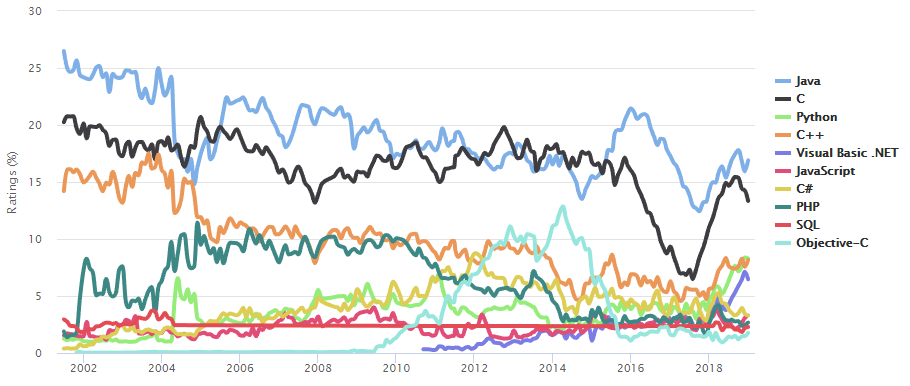
\includegraphics[width=1.0\linewidth]{PICs/lang_ratings}
	\caption{Most popular programming languages throughout the years \mcpic{lang_ratings}.}\label{lang_ratings}
\end{figure}
 This is however where OOP and modern computer architectures do not get along, so to say. OOP offers an elegant way to intuitively model an issue into code, but doing so it encourages us to implement our data in an inefficient way. Inefficient because creating monolithic models of our data usually lack cohesion, which means, that the classes' members tend to not be related/dependent \mc{cohesion} - at least in terms of computational order or domain affiliation. In a home office application, juggling a few dozens of entities every other minute, this will not appear as a problem. And in this case it might be preferable to program such application in a strict object oriented way, since the development can be done fast and reliably even by a novice. On the other hand and especially in the game development industry OOP has proven to result in poorly performing software, due to inefficient data layouts. Because especially for games where oftentimes lots of game entities are being processed several times per second: "\textit{data is performance}" \mcp{nystrom}{272}.\\
 \begin{lstlisting}[language=C++,numbers=none,name={Example of some hierarchical POD class definitions},label={pods}]
struct Obj {				struct Human : Obj {			struct NPC : Human {
	float xyz[3];				char *name;						int mood;
	float vel[3];				int age;						};
};								};

NPC npc_arr[3];
 \end{lstlisting}
The abbreviation \textit{AOS} stands for \textit{Array Of Structures}\mc{intel} and it describes, what usually happens with Object Oriented Programming.\\
Considering the rather arbitrary C++ class definitions in \refcode{pods} the \textit{npc\_arr} will occupy memory according to \reffig{npcs_in_memory} (disregarding any \textit{padding}).
\begin{figure}[!htbp]
	\centering
	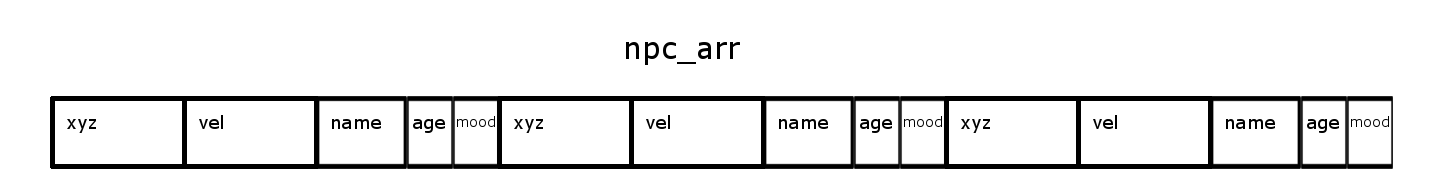
\includegraphics[width=1.0\linewidth]{PICs/npcs_in_memory}
	\caption{Visualization of how \textit{npc\_arr} will exist in memory}\label{npcs_in_memory}
\end{figure}
This is quite literally an array of structures - hence the notation \textit{AOS}. The following sections \ref{cpu_caches} and \ref{dod} will elaborate on \textit{why} exactly this way of thinking/way of abstraction and its respective layout in memory is inefficient.

\section{CPU Caches and why they don't \textit{fit} objects}\label{cpu_caches}
The data layouts typically found when programming with objects and classes, are not inefficient because they lack logic. "\textit{Each human - including NPCs - will have positional traits}", is semantically correct. In fact it seems rather unfortunate, that modern computer architectures ca not deal well with an abstraction that fits our perception of the world. But the hardware is not to blame here. The problem with monolithic class definitions is much more that of common coding- or data access patterns.\\

\subsection{Common data access patterns vs. Monolithic class definitions}\label{cdap}
Numerous coding best practices teach us to write simple, modular code.
\begin{quote}
	\textit{Functions should do one thing. They should do it well. They should do it only.} \mcp{rcmartin}{35}
	
	\textit{Keep it simple and smart} (KISS principle). \mcp{niemann_kiss}{77}
	
	\textit{[...] cohesion is an important object-oriented
		software quality attribute.}\mc{cohesion}
\end{quote}
Just like we want our class definitions to share a common responsibility or task, we want the set of instructions that iterate and probably transform a set of data to be as simple and modular as possible. So usually we try to not write monolithic \textit{for-loops} handling every single aspect of a set of data.\\ For example in \reffig{npcs_in_memory} we would not want a loop that handles each and every single member of an NPC. This would not only result in a big set of instructions, that hides the individual purposes of each expression, but also make it hard to maintain/change the code. Not to mention, that different data often demands change at different times at runtime. Requirements can change quickly. Breaking up responsibilities that were coupled and forced to coexist change not so quickly.\mc{rcmartin}\\
Exemplary if \refcode{pods} was the model for a game, our game loop could at one point iterate over all the elements in the \textit{npc\_arr} to update their position and velocity for each frame. The \textit{NPC's mood} could just as well be updated frequently in a separate function, that only encompasses the information relevant for the calculation of the updated mood.
Their \textit{Human::name}s however will most likely not change so frequently - if ever - so the instructions to modify that data will most likely depend on user input and exist in yet a whole other routine. This modularization of code is commonly referred to as \textit{Separation of Concern} and has proven to improve the code's maintainability \mcp{laplante}{85}.
\textit{This} keeping the objects in some sort of set, then iterating over it for each routine, that manages a subset of the object's data, is a common access pattern that is applied on objects in OOP.\\
The interim conclusion here is, that even only for maintainability reasons, it is desirable for programmers to process logically related subsets of their data separately - but then why is the resulting software so slow compared to the same idea implemented with a \textit{Data oriented Design}?\\
The Object Oriented Programming paradigm is exactly doing what it promises - providing a sort of abstraction, that programmers can intuitively apply to their problem definition. Consequently OOP programmers quickly adapt the habit of developing against their abstraction because it is intuitive. What is lost in the process is the concern of developing against the rationale and thinking about how it interacts with the hardware. \textit{This} is probably the fundamental difference between OOP and DoD.\\
So whats our hardware's deal? Why do objects don't get along with it. Why can't we have super high speed machinery, that makes hardware concerns obsolete? Why can't we have anything nice?
In conclusion the key question seems to be why objects don't utilize hardware components  optimally. Also are there not any high speed memory units available by now, which could help making hardware concerns obsolete?

\subsection{A brief history of memory}
To answer \refsec{cdap}'s concluding question: There are high speed memory units at hand but they are cost-intensive. Modern computer systems rely on a variety of different memory units each differing in access latency, capacity and numerous technical properties. The intention behind this complex hierarchy of memory layers is of course speed and is the result of an evolving cost-benefit calculation.
\begin{quote}
	\textit{The task the computer designer faces is [...] design a computer to maximize
		performance while staying within cost[...].} \mcp{hennessy}{8}
\end{quote}

Originally
\begin{quote}
	\textit{memory access latency and instruction execution latency were on roughly equal footing. [...] register-based instructions could execute in two to four cycles, and a main memory access also took roughly four cycles.} \mcp{gregory}{189}
\end{quote}
This proportion changed significantly. While it is relatively cheap to produce high speed CPUs, this is not the case for memory units. So whats happening, is that today's PCs/consoles are equipped with CPUs that are way faster than the greater parts of their available memory units. Due to increasing tick rates and \textit{Instruction Pipelining} what used to be ~four cycle RAM reads are now several hundred cycles. Not Because RAM became slower - the opposite is the case - but because CPUs became that much faster in relation.
This trend was thoroughly observed and documented by John L. Hennessy and David A. Patterson \reffigp{cpu_memory_gap}.\\
\begin{figure}[!htbp]
	\centering
	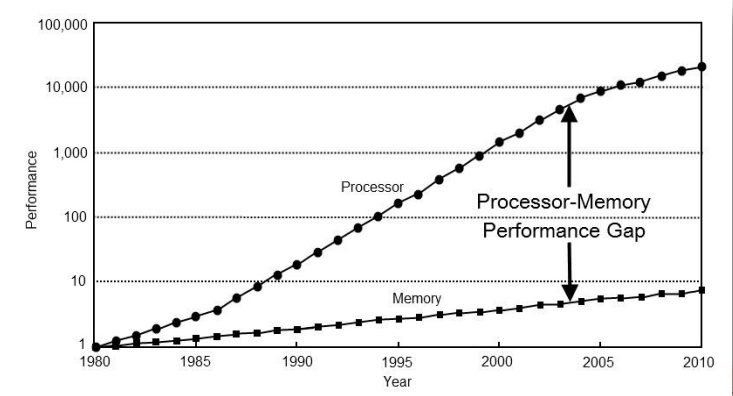
\includegraphics[width=0.7\linewidth]{PICs/cpu_memory_gap}
	\caption{"\textit{\textbf{Starting with 1980 performance as a baseline, the gap in performance
			between memory and processors is plotted over time}.
			Note that the vertical axis
			must be on a logarithmic scale to record the size of the processor-DRAM performance
			gap. The memory baseline is 64 KB DRAM in 1980, with a 1.07 per year performance
			improvement in latency (see Figure 5.13 on page 313). The processor line assumes a
			1.25 improvement per year until 1986, and a 1.52 improvement until 2004, and a 1.20
			improvement thereafter}" \mcppic{hennessy}{289}}\label{cpu_memory_gap}
\end{figure}\\
To solve the issue of ever diverging CPU/memory performances (commonly referred to as the \textit{memory gap \mcp{gregory}{189}}), specifically to reduce the latency of references to main memory, smaller but significantly faster (and more expensive) memory units are placed between the CPU and the main memory. These modules are called \textit{Caches} - first named by C.J. Conti \mcp{conti}{15} in 1969. Originally cache technology was mentioned as \textit{buffers}\mcp{cragon}{15}. Not considering their complex, modern modalities and policies this is a fitting notation.\\
The basic idea behind a fast buffer interconnected between the CPU and the main memory is to create local copies of referenced data-chunks, in order to provide faster access on subsequent calls to the same \textit{AU} (Adressable Unit) as well as the ones deemed likely to be accessed soon \mcp{gregory}{191}. This principle originated in the work on \textit{Virtual Memory} \mcp{cragon}{15} and is today much more sophisticated.\\
So high speed memory actually exists in our common computer architectures, those particular components are however limited due to their cost intensity and physical barriers.

\subsection{Cache modules and types}
In today's PCs/consoles typically each CPU core has its own hierarchy of cache modules \reffigp{cache_layout}.
\begin{figure}[!htbp]
	\centering
	\includegraphics[width=0.4\linewidth]{PICs/cachelayout}
	\caption{Exemplary, simplified model of a CPU core and its several cache modules \mcppic{Drepper}{15}}\label{cache_layout}
\end{figure}
Closest to the core (on-chip) is the \textit{L1} (Level 1) cache. Accessing an AU in the  Intel i7 Processor's L1 cache for example is almost as fast as accessing it in the very CPU's registers - ~4 cycles (2.1 to 1.2 ns) \mc{levinthal}. For reference access to main RAM "\textit{can take on the order of 500 cycles[...]"} \mcp{gregory}{189}.
Another cost unrelated reason, why there is not lots of \textit{L1 D} cache is that more memory means literally more physical space is occupied. Having more cache memory equals more \textit{cache hits} \refsecp{cpucu} but as soon as the cache can not fit on-chip anymore, there is yet again additional latency. That is why the L1 and sometimes L2 cache modules are kept comparably small but on-chip. Other L3 and L4 caches are each bigger and slower than their preceding counterparts respectively, but for the most part share the same ideas slowly converging latency times to the common main memory RAM.\\
CPU cores can share one or more cache modules (usually starting with L2 or L3), effectively accessing the same local copies of data. This entails synchronization issues as the overlying smaller and faster cache-modules may not work on diverging information.\\
Modern cache hierarchies include data caches as well as instruction caches, usually both in an L1 cache. However there are different takes on how to implement this. Harvey G. Cragon lists \mcp{cragon}{17}:
\begin{itemize}
	\item instruction cache - holds only instructions
	\item data cache - holds only the data stream
	\item unified cache - holds both instructions and data
	\item split cache - two-cache system, one for instructions and one for data
\end{itemize}
While optimizing against better instruction cache utilization can result in significant performance boosts \refsecp{conclusion}, the scope of this masters thesis will omit instruction-cache related subjects, because the upcoming attempts and techniques to achieve performance optimizations will focus on improving the data layout of a given target source code.
%local  L1 CACHE hit,                              ~4 cycles (   2.1 -  1.2 ns )
%local  L2 CACHE hit,                             ~10 cycles (   5.3 -  3.0 ns )
%local  L3 CACHE hit, line unshared               ~40 cycles (  21.4 - 12.0 ns )
%local  L3 CACHE hit, shared line in another core ~65 cycles (  34.8 - 19.5 ns )
%local  L3 CACHE hit, modified in another core    ~75 cycles (  40.2 - 22.5 ns )
%remote L3 CACHE (Ref: Fig.1 [Pg. 5])        ~100-300 cycles ( 160.7 - 30.0 ns )

\subsection{The CPUs cache utilization}\label{cpucu}
A programmer will rarely ever directly interact with a cache module (though there are mechanisms for manual prefetching/clearing). The underlying idea for it was to be transparent to the programmer. However understanding the CPUs cache utilization enables one to tailor the data layout to it, resulting in faster access, less waiting and consequently higher throughput. Among other things, this is what \textit{Data oriented Design} aims to do - developing against hardware concerns. \mcp{fabian}{268}\\
As mentioned before the basic idea of the cache is to provide local copies of data at a faster rate and prefetch data segments, that are likely to be used soon. This works by directing each main memory access to go through the cache. Main memory access means also going through virtual address translation, address and data buses and depending on the main memory, crossbar switching logic \mcp{gregory}{190}.  
Whenever the CPU requests access to a certain AU before saddling the horses and going on a journey to main memory, the cache will check whether or not the requested AU is currently present inside its buffer. If so it is referred to as a \textit{cache hit}, otherwise a \textit{cache miss}. For a modern L1 D cache this buffer, to be more specific, consists of several cache lines usually each of 64 bytes. Overall cache- and line sizes vary between different architectures and levels but are standardized mostly due to Intel's designs.\\
Cache misses result in higher access latency and should be avoided if possible. It is however not always possible. \textit{Mark Donald Hill} describes three classifications for cache misses \mcp{hill}{50}:
\begin{itemize}
	\item Compulsory Miss - Access to previously unreferenced data blocks. E.g. the very first data access will inevitably result in a main memory access.
	\item Conflict Miss - Due to data blocks mapping to the same cache-lines.
	\item Capacity Miss - Due to the cache's finite capacity. Lots of data accesses will eventually displace older/less-used entries in the cache (depending on Replacement policies).
\end{itemize}
The simplest and least efficient implementation to determine a cache \textit{hit/miss} is to iterate each cache line comparing fitting criteria. To prevent this nowadays caches implement a certain associativity technique. This way each individual physical main memory address can be mapped to one or more specific cache lines. Doing so addresses are converted to and managed by metadata consisting of: \mcp{gregory}{193}
\begin{itemize}
	\item Offset - Offset to the actual referenced Byte inside the cache line.
	\item Cache Line Index - Which cache line/s would hold the AU.
	\item Tag - Which cache sized block in main memory holds the original data.
\end{itemize}
In the case that each physical main memory address has exactly one counterpart it is called a \textit{direct-mapped} cache \mcp{gregory}{194}. In this case since the cache can by far not encompass the whole extend of the main memory, a lot of physical addresses will be mapped to the very same cache line, effectively extruding each other out of the cache when accessed. This is called \textit{eviction} and in unlucky cases will behave like all references are cache misses \mcp{cragon}{97}. To prevent this modern caches map a physical address to \textit{n} cache lines. This is described as \textit{n-way associativity} - typically implemented as \textit{8-way} or \textit{16-way} caches depending on the level.\\
There is a lot more to cover about caching technologies and policies like: Replacement-/Write-/Coherency(MESI; MOESI; MESIF) policies and for further reading Harvey G. Cragon's \textit{Memory Systems and Pipelined Processors}\mc{cragon} as well as Jason Gregory's \textit{Game Engine Architecture}\mc{gregory} are highly recommended. However for the purpose of this work a few specifics are most interesting.\\
How can a data layout affect \textit{hit ratios} and reduce calls to main memory? As mentioned before there are common data access patterns in software and the caches actually accommodate us by adapting their builtin prefetching mechanisms to it, following a set of \textit{locality concepts}. Harvey G. Cragon counts three of those concepts: \mcp{cragon}{16}
\begin{itemize}
	\item \textit{Temporal locality} - Information recently referenced by a program is likely to be used again soon.
	\item \textit{Spatial locality} - Portions of the address space near the current locus of reference are likely to be referenced in the near future.
	\item \textit{Sequential locality} - A special case of spatial locality in which the address of the next AU will be the immediate successor of the present one.
\end{itemize}
At first glance these concepts are very straight forward, but their respective implementations for automatic hardware prefetching can be more complex than one would think. Prefetching data basically means:
\begin{quote}
"\textit{[...] bringing data in the data (or mixed instruction-data) cache before it is directly accessed by a memory instruction [...].}" \mcp{chen}{610}
\end{quote}
There are however different strategies to decide which bytes should be faithfully loaded into the cache. Tien-Fu Chen and Jean-Loup Baer list two categories for prefetching strategies: \mcp{chen}{610}
\begin{itemize}
	\item \textit{Spatial} - access to current block is basis for prefetching.
	\item \textit{Temporal} - lookahead decoding of instruction stream is implied.
\end{itemize}
There are simple approaches like: whenever block \textit{i} is accessed, prefetch block \textit{i}+1, called the \textit{One Block Lookahead}; stride based approaches storing previously referenced addresses in a table and calculating a stride based on current and previous addresses; combinations of both and many more \mc{chen}.  Sometimes data is prefetched into the cache, sometimes into separate stream buffers. There are many different hardware prefetching methods to find and while data cache prefetching is considered to be more challanging \mcp{mittal}{4} it is still best practice to rely on spatial locality when modeling data to play into the cache's hand.\\
Compilers already make use of software prefetching (manual cache interaction instructions) in certain cases.
\begin{quote}
	\textit{For array-based applications, the compiler can use locality analysis to predict which dynamic references to prefetch, and loop splitting and software pipelining to schedule prefetches.} \mcp{luk}{223}
\end{quote}
So we can already deduce that for an efficient data layout it would be beneficial to rely on arrays, or more generally, concepts compilers can 'comprehend' and optimize. Also even though the concept of \textit{sequential locality} is only a special case, it is the one we can utilize best to derive adaptations for our data layout, since hardware prefetching has adapted best to it. DoD converts this information into a generic set of rules/best practices, a methodology for efficiency.

\section{Data Oriented Design}\label{dod}
The whole purpose of adding abstraction layers is moving further away from the hardware mentally. This helps us to focus on constructing appropriate models for a problem \mcp{kramer}{5}. However disregarding intrinsic detail is predestined to result in poor resource utilization at that level. \textit{Data oriented Design} wants us to be aware of what is beneath the source code and tailor the essential resources to it. Essential resources here being our data. 
\begin{quote}
	\textit{The data-oriented design approach doesn't build the real-world problem into the code. This could be seen as a failing [...] by veteran object-oriented developers [...]. [It] gives up some of the human readability [...], but stops the machine from having to handle human concepts [...].} \mcp{fabian}{7}
\end{quote}
\subsection{OOP and bad abstraction}\label{oop_bad_abstraction}
DoD however deserves more credit than only being a performance optimization. (Wrong) abstraction not only moves us away further from the hardware, but also from the actual problem domain.\\
Even though \textit{coupling} and its avoidance are a big deal in OOP it somehow seems natural to couple the data and the problem domain. This coupling has proven to lead to the exact same problems as coupling of unrelated classes. Its hard to make changes, especially when the reason for change is modification of fundamental design choices. But not only is contextual linkage rigid to conceptual change but its also hard to operate on it only in ways that haven't been thought of initially.\\
Imagine for example a simple particle system implemented in a typically OOP manner \refcodep{particle_system}.

 \begin{lstlisting}[language=C++,name={ OOP typical, simplified particle system implementation},label={particle_system}]
struct particle
{
	float ms_alive, lifetime_in_ms, xyz[3];
	Shader *shader;
};

struct particle_system
{
	particle particles[1024];
	unsigned particles_alive;
	...
};
\end{lstlisting}
At first glance it appears to be a perfectly valid approach to make a particle system linked directly to the very particles it is supposed to manage (\refcode{particle_system} line 10). Each method will now operate on the particles array and just like that we can make numerous particle systems, each implicitly operating only on its own data. This is an easy to grasp concept that in terms of a particle system we could easily match with a real-world fireworks battery. In regards of maintainability there is already a huge issue.\\
Concerning operations, that need to be applied to all particles right now this implementation does not provide an easy solution to do so. When in the real world do two physically different particle systems ever interact with each other? Collision might come to mind. While it would be a lot easier to just iterate a big list of particles, we don't really care. It is still relatively easy to just check each particle system's particles against another particle system \refcodep{collision}. And we will just do this for all the particle systems we have! They probably should exist somewhere in the same context anyway.\\
 \begin{lstlisting}[language=C++,name={Example code how OOP could handle collision between different particle systems' particles},label={collision}]
void particle_system::particle_system_collision(
	particle_system *ps1,
	particle_system *ps2)
{
	for(unsigned i = 0; i < ps1->particles_alive; ++i)
	{
		particle *p1 = &ps1->particles[i];
		for(unsigned o = (ps1 == ps2 ? i+1 : 0); o < ps2->particles_alive; ++o)
		{
			particle *p2 = &ps2->particles[o];
			[collision code]
		}
	}
}
\end{lstlisting}
Even though \refcode{collision} has some uncomfortable specifics (especially line 8), it is still doable. The moment we start to render this particle system however one might notice that the particles are occasionally blurry. The particles' sprites make use of transparency and even though transparency is enabled in the render back-end it doesn't look right. For transparency to be applied correctly,the particles need to be rendered in a certain order. This circumstance might have not occurred to the programmer while designing the data model. It is easy enough to sort one particle system's particles according to their distance to camera respectively, but bringing EACH particle system's particles in order?\\
One could write an algorithm, that has a list of particle arrays; takes each particle system's particle array; unifies them to a big dynamically allocated array; then sorts it; then returns that array so it can be rendered. Each frame. This also implies changing the render pass, since now it is not the particle systems to render but one big array of particles.\\
These changes are starting to proliferate really fast. One does not have those sort of issues with a real-world fireworks battery and might feel betrayed by the abstraction to it. Ultimately we come to a point where we understand, that a real-world projection of a problem domain into source code might not be the best choice. Its definitely possible, but does not provide the optimal attempts to solve the problems specific to certain tasks. So instead of realizing overly complex solutions to make our code fit our abstraction we realize that our abstraction is obsolete and we should focus on a solution that fits our tasks. In the end data is not generic in the way it is used\mcp{fabian}{15}. Different jobs might require different solutions and OOP might be optimal for a subset of problems, but has evolved into a pattern, that is forced on domains as a go to.\\
Besides additional layers of abstraction do not equal superior usability/readability either. When using a third party library we hope the API designer provides functions that operate on data types we are already familiar with, like char pointers, instead of forcing us to learn how to use that developers self-made string class (KISS).\\\\
So arguably Object Oriented Programming is not automatically superior, neither in terms of maintainability nor performance. Actually it appears to be inferior to DoD. So the question is: What does DoD do to be \textit{better}?\newpage
\subsection{Normalization of Data}
When thinking in terms of the problem and designing against the data \textit{Richard Fabian} references relational database models as a worthy category to look up to in his book \textit{Data-Oriented-Design: Software engineering for limited resources and short schedules} \mcp{fabian}{25}. After all a database should handle data correctly.\\
We have already seen, that the object typical data-layout makes sense in terms of readability, but fails to be maintainable and in terms of cache utilization behaves poorly. In order to peel off of the OOP abstraction pattern we want our model to be a minimal, precise representation, that abides a format, that has proven to behave well. Fabian says:
\begin{quote}
	\textit{The structure of any data is a trade-off between performance, readability, maintenance, future proofing, extendibility, and reuse.} \mcp{fabian}{28}
\end{quote}
Therefore we could attempt to treat our data modeling process the way we would, when setting up a relational database. We normalize our data, according to the existing normalization stages developed by Edgar F. Codd and Raymond F. Boyce \mc{codd}. This is done because laying out your data in a linear fashion goes away from embedding meaning to its structure (Class/Struct) \mcp{fabian}{25} and has proven to give advantageous insights to the data, its domain and the relations between its subsets. Dealing with the problem's domain and the underlying data eventually led to technologies like JPEG and MP3 \mcp{fabian}{47}. Understanding the data will lead to an understanding of the solution.
\begin{table}[H]
	\centering
	\scalebox{0.7}{
	\begin{tabular}{@{}lllllll@{}}
	\toprule
	\textbf{particle\_id} & \textbf{shader\_id} & ms\_alive & lifetime\_in\_ms & x   & y    & z     \\ \midrule
	p0                    & s0         & 7034      & 10000            & 4.0 & 10.1 & -12.9 \\
	p1                    & s0         & 122       & 10000            & 0.5 & -8.1 & -2.6  \\
	p2                    & s0         & 4310      & 10000            & 1.1 & 7.4  & -3.0  \\
	...                   &            &           &                  &     &      &       \\
	p1024                 & s1         & 86        & 100              & 7.0 & 0.0  & 0.5   \\
	p1025                 & s1         & 44        & 100              & 3.0 & 0.0  & 0.2   \\
	... &&&&&& \\
	\bottomrule
	\end{tabular}}
\end{table}
\begin{table}[H]
	\parbox{0.5\linewidth}{
		\centering
		\scalebox{0.7}{
		\begin{tabular}{@{}cll@{}}
			\toprule
			\textbf{system\_id} & particles\_alive\\ \midrule
			ps0                 & 462                   \\
			ps1					& 99				   \\ \bottomrule
		\end{tabular}}
	}	
	\parbox{0.5\linewidth}{
		\centering
		\scalebox{0.7}{
		\begin{tabular}{@{}cll@{}}
			\toprule
			\textbf{system\_id} & \textbf{particle\_id}\\ \midrule
			ps0                 & p0                   \\
			ps0                 & p1                   \\
			ps0                 & p2                   \\
			...                 &                      \\
			ps1					& p1024				   \\
			ps1					& p1025				   \\
			... & & \\ \bottomrule
		\end{tabular}}
	}

	\caption{Example excerpt of a possible first normalization step for the particle system and how it indicates bad design}
	\label{normalized_ps}
\end{table}
For our minimal example of a particle system, even just the first stages of normalization teaches us, that there should be no arrays of data in one element \mcp{fabian}{37} it also forces us to reconsider which data is accessed through which instance (key) and therefore whether or not there is a \textit{relation} to find \reftablep{normalized_ps}.\\We will not implement a relational database for our application but generating this model can help us realize some things.
\begin{enumerate}
	\item particles are no longer represented block-wise, but are held in ONE unified table to begin with.
	\item Instead of holding an array of particles we can just as well take its data subsets and link them against a unique key, which basically translates to each member is a column/array and each instance of a particle or particle system is now a mere index.
	\item There is tons of redundancy. Not logical but contextual. Seeing the same \textit{shader\_id} and \textit{lifetime\_in\_ms} over and over for each particle that will share a particle system certainly \textit{smells} funny. It is very important to be able to link each particle to a specific shader, but contextually this is redundant. We can see, that some things might have been coupled due to our abstraction.
	\item Especially after resolving redundancy, rethinking which data belongs to which entity hints at \textit{when} specific subsets are accessed and in which context (which key is used to get it) encouraging us to implement domain wise processing of an entities attributes.
\end{enumerate}
After \textit{laying out our data} in a linear fashion, we can now implement a \textit{data layout} that implements our new ideas.

\subsection{Structure of Arrays / SOA}\label{soa}
In contrast to the previously mentioned AOS \refsecp{OOP} a \textit{Structure of Arrays} (SOA) is the \textit{column-oriented database} pendant to a data layout that results in higher throughput by providing a cache friendlier structure \mcp{fabian}{163}. We already know now, that the hardware, specifically the cache uses certain strategies to provide data out of main memory, that is likely to be used soon. This happens both when loading data in cache-line sized blocks and through prefetching mechanisms \refsecp{cpucu}. Now when implementing the column-oriented approach that comes with data normalization we automatically almost perfectly conform to those auxiliary means by implementing columns as arrays. The original concept of an \textit{object} can now be simplified to an index, that retrieves the respective values in each column/array.\newpage
\subsubsection{AOS in the cache}
\begin{wrapfigure}[11]{r}{.35\textwidth}
\vspace{-1cm}
\begin{lstlisting}[language=C++,numbers=none,name={NPC pod after derivation is done},label={post_deriv_npc}]
struct NPC 
{
	//inherited from Obj 
	float xyz[3];
	float vel[3];
	//inherited from Human
	char *name;
	int age;
	//NPC
	int mood;
};
\end{lstlisting}
\end{wrapfigure}
Remembering \refcode{pods}, when examining the NPC class we know that after derivation (done by the compiler) it looks like \refcode{post_deriv_npc}. Accessing subsets of an instance of NPC will always result in loading at least a whole cache line. Let us assume, that the game code will iterate over the NPCs to update their positions by adding their velocity multiplied with a delta-time to their current xyz. With a typical L1 D cache-line of 64 Byte and assuming that an NPC is 40 Byte (float = 4 Byte, pointer = 8 Byte) we can make the following assumptions: Considering the subset of data we actually want to work with on our update routine per NPC is $2\times 3\times \textit{sizeof(float)} = $ 24 Byte, we waste $40 - 24 =$ 16 Byte of our cache per NPC. Due to our algorithms complexity \refsecp{asymptotic_notations} this waste scales linearly with our data.\\
As a quick approximation onto a damage report we could do the following:
The smallest common multiple of our 40 Byte NPC and our 64 Byte cache-line is 320, so with eight NPCs we load five cache-lines \reffigp{cache_utilization_npc}. This equals five compulsory misses. After 320 Byte this layout repeats so we could extrapolate to greater numbers of NPCs \reffig{soa_aos_cl_usage}. 
\begin{figure}[!htbp]
	\centering
	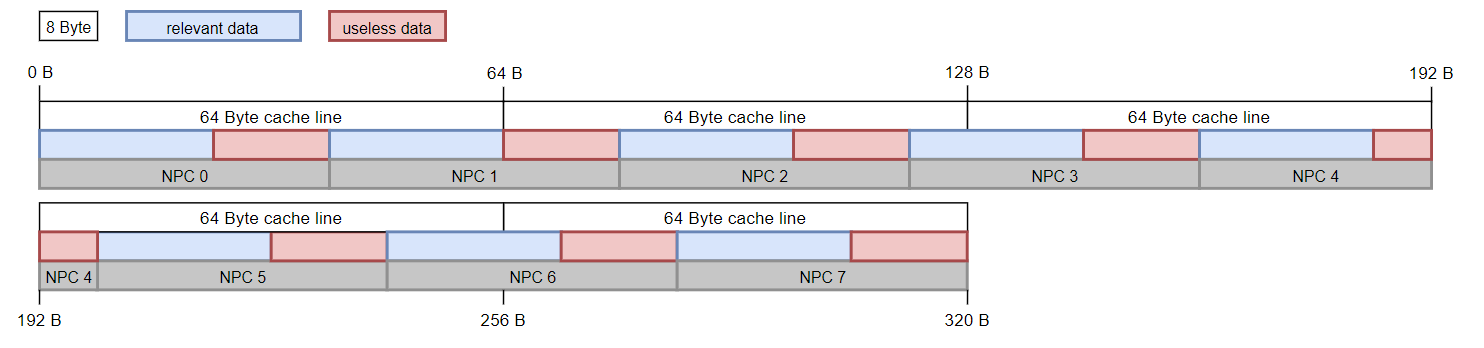
\includegraphics[width=1.0\linewidth, height=0.3\linewidth]{PICs/CacheUtilizationNPC}
	\caption{NPCs inside cache-lines, where blue is relevant data and red blocks represent unused data}\label{cache_utilization_npc}
\end{figure}
A cache miss occurs whenever we do not find an AU inside a cache line. While \textit{NPC0} completely fits inside the first cache-line, \textit{NPC1} does not. However \textit{NPC1}'s relevant data also completely fits in the first cache-line, so accessing it's relevant data will not result in a cache miss! While accessing \textit{NPC2}'s relevant data will partly load \textit{NPC3}'s relevant data, we will only get the first eight Byte of it. The remnant will be loaded separately, yet this will result in completely loading \textit{NPC4}'s relevant data.\\
Continuing this we will count five cache misses and foregoing from 320 loaded Bytes this process will repeat. The statement that 1000 NPCs will count $1000 npc = \frac{5 * 1000}{8} cms = 625 cms
$ cache misses for the position update routines (where \textit{cms} are cache misses), is only a narrow assumption, since our cache-lines are defined in fixed quantums \reffigp{soa_aos_cl_usage}.
\subsubsection{SOA in the cache}
\begin{wrapfigure}[9]{r}{0.4\textwidth}
\begin{lstlisting}[language=C++,numbers=none,name={SOA variant of the NPC},label={soa_npc}]
struct NPCs{
	float xyz[3 * NUM_ENTITIES];
	float vel[3 * NUM_ENTITIES];
	char *name[NUM_ENTITIES];
	int age[NUM_ENTITIES];
	int mood[NUM_ENTITIES];
} npcs;
\end{lstlisting}
\end{wrapfigure}
Implementing the \textit{NPC} in a SOA manner it could look like \refcode{soa_npc}. What used to be individual class members are now columns/arrays, accessed by a key - the \textit{npc\_id}. From now on both reads to \textit{xyz} and \textit{vel} will fill a cacheline worth of relevant data, respectively. A single cache-line now holds up to five ($5\frac{1}{3}$) positions or velocities. This doesn't prevent our data from overlapping in terms of cache-lines. The smallest common multiple of 12 and 64 is 192, so over $\frac{192}{64}=3$ cache-lines we will fit $\frac{192}{12}=16$ units. As can be seen in \reffig{soa_aos_cl_usage} the SOA attempt will develop better cache utilization for contiguous AU access on rising data sizes, disregarding any external eviction. This does not automatically equal the amount of cache misses, since repeated data access will find the data in the cache. But a SOA data model will reduce compulsory misses.
\subsubsection{}
\vspace{-1cm}
\begin{wrapfigure}[16]{l}{.6\textwidth}
	\centering
	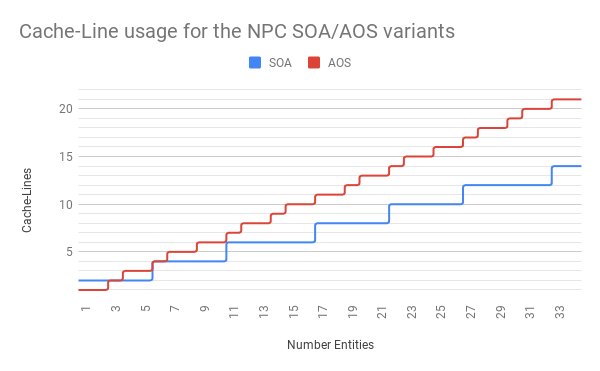
\includegraphics[width=.6\textwidth, height=0.42\textwidth]{PICs/soa_aos_cl_usage}
	\caption{Cache-line efficiency comparing NPCs represented as SOA and AOS.}\label{soa_aos_cl_usage}
\end{wrapfigure}
The unit we use for computations here is the size of three floats (12 Byte), so while a cache-line fits $\myfloor{\frac{64}{12}}=5$ complete units, the remnant of $64-12\times5 = 4$ Byte will belong to a unit, we will need another cache-line for. This overlap happens exactly $\frac{12}{64-60} = 3$ times until in the fourth cache-line this process repeats. Distributing logically dependent data over multiple cache-lines should be avoided, since access to it will result in more cache misses and is prone to eviction \mcp{intel}{12-19}.\\
It can be solved by adjusting the data's \textit{alignment}. Since this will be used in the prototypical implementation it will be explained in section \ref{memory_management}, for now we could assume, that we align and pad our \textit{float[3]} blocks of data to our cache-lines in a way that each cache-line holds exactly five of those entities \reffigp{cache_utilization_soa}.\\
This leads to consistent throughput. In numbers we now have exactly two cache misses per five \textit{NPCs} (We don't really have an NPC object anymore, but we are still allowed to \textit{think} in objects). One for the positional data, one for the velocity data. Again for 1000 NPCs this would now result in 400 cache misses what translates to $225\times\sim300$ clock cycles less latency than the AOS version, for position updates alone! Each frame!
\begin{figure}[!htbp]
	\centering
	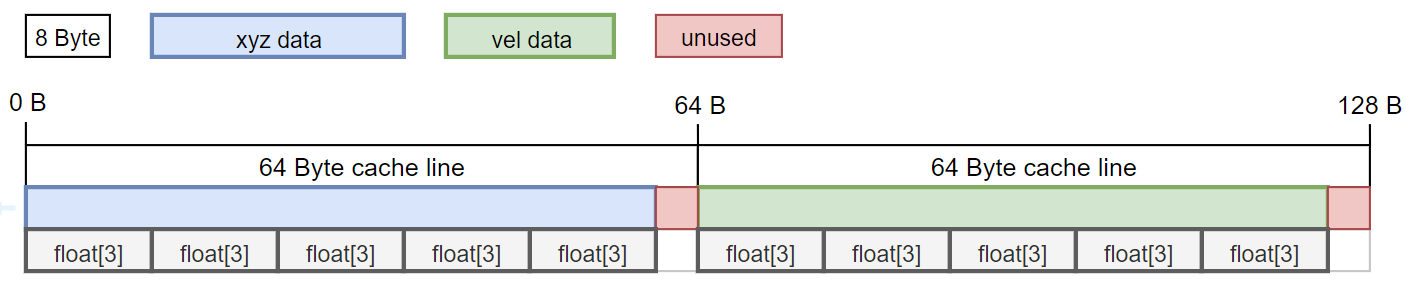
\includegraphics[width=1.0\linewidth, height=0.17\linewidth]{PICs/CacheUtilizationNPCSOA}
	\caption{xyz and vel blocks inside cache-lines, where blue represents joint float[3] blocks of xyz data, green joint blocks of float[3] vel data and red is unused but intentional padding.}\label{cache_utilization_soa}
\end{figure}
This is starting to behave \textit{optimal}. By not loading unneeded data into the cache we can store more relevant data. By Aligning and padding our data blocks correctly we attenuate the chance of \textit{conflict misses} since we reduce the number of cache-lines the related data depends on. We do however still have leftover space. The four Byte paddings we append to each $5\times float[3]$ block has purpose, yet could theoretically hold information. Imagine our now theoretical NPC and thus our positional computation would involve a per NPC factor for maybe damping, as well as a mass. Still assuming that $sizeof(float) = 4$ this would be an additional eight Byte per NPC on each computation. Following our SOA approach we would define yet two new arrays for the damping factor and mass respectively. Accessing them would result in the utilization of another two cache-lines. Even though those cache-lines now suffice 16 NPCs each ($\frac{64}{sizeof(float)} = 16$) we now are dependent on four individual cache-lines to compute the \textit{update\_npc\_position} for one NPC, so the amount of cache-lines scales linearly with the amount of parameters the computation depends on (for SOA). In terms of eviction and consequently of conflict misses, this could yet again cultivate sub-optimal cache utilization (for the same reasons Intel's article on \textit{Memory Layout Transformations} \mc{aosoa} also mentions increased pressure on the \textit{TLB} (Translation Look-aside Buffer)). Even though we reduced the overall NPC per cache-line ratio, there is still unused information and scaling prone to eviction, all due to the individually related data blocks being physically separated. This doesn't countermand that SOA performs better than AOS, but it indicates that it might only be optimal for certain types of computations (e.g. SIMD) there is still room for improvement.\\\\
Note that while SOA greatly fits SIMD it is not considered to be an ideal solution to encompass objects \mcp{gregory}{1060}. For that we need solutions, that regard both temporal and spatial locality. 

\subsection{Regarding temporal- and spatial locality}\label{rtasl}
The motivation behind our AOS to SOA conversion, was to maximize cache utilization when processing an NPC's position. We figured, that loading an object entails lots of unwanted data that does not share temporal locality with the information that is relevant to us. So we made sure, that instead of objects we loaded only wanted data.
\begin{wrapfigure}[10]{r}{0.4\textwidth}
\begin{lstlisting}[language=C++,numbers=none,name={Consolidating related data},label={component_npc}]
struct npc_group{
	float xyz[3];
	float vel[3];
	float mass, damping;
};

npc_group npc_groups[NUM_ENTITIES];
\end{lstlisting}
\end{wrapfigure}
In order to do so we gave up something very important. When data is logically related it means, that it collaborates/is involved in the same data transformations. Whenever we see, that certain subsets of data are frequently used together it is advisable not to separate them. So instead of rigorously converting each member into an array pendant, we group logically related data and create arrays of those groups instead \refcodep{component_npc}.This way the relevant data concerning one NPC will not spread over different incoherent cache-lines, that could map to completely different segments in main memory.\\\\
This technique bundles related data and makes sure it is successive in memory as well as in cache-lines, consequently we won't peril those cache-lines to extrude each other from the 
\subsubsection{}
\vspace{-1cm}
\begin{wrapfigure}[8]{l}{0.37\textwidth}
	\vspace{-0.4cm}
	\centering
	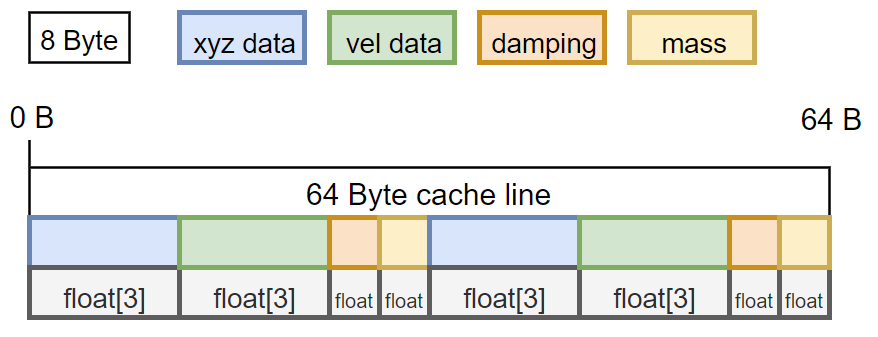
\includegraphics[width=.37\textwidth, height=0.17\textwidth]{PICs/CacheUtilizationNPCComp}
	\caption{Unified/Grouped relevant data in a cache-line.}\label{cache_utilization_comp}
\end{wrapfigure}
cache. The book \textit{Compilers, Principles, Techniques and Tool} also describes a mechanism like this and refers to those groups as \textit{blocks} \mcp{aho}{786}.
Also we get the chance to fully exploit our hardware's boundaries, as in now we can get rid of manually inserted padding Bytes \reffigp{cache_utilization_comp} - provided we have related data that fits the gap. It is however only possible to gain a performance boost out of this, when the unified data shares temporal locality.

\subsubsection{Hot/Cold Splitting}\label{hot_cold_splitting}
\begin{wrapfigure}[15]{r}{0.3\textwidth}
\begin{lstlisting}[language=C++,numbers=none,name={The NPC class splitted into hot/cold data},label={hcsplit_npc}]
struct npc_cold_data{
	char *name;
	int age;
	int mood;
};

struct npc{
	float xyz[3];
	float vel[3];
	npc_cold_data *cold_data_ptr;
};
\end{lstlisting}
\end{wrapfigure}
A famous practical application of grouping a particular subset of data is called a \textit{Hot/Cold Split} \mcp{nystrom}{283}. It is also used to improve cache utilization, it only has a very specific definition of what members should be grouped.\\
The idea is to separate a record's member definitions into two subsets. One that contains all the hot-, and one that contains all the cold members respectively. Data is hot when it is used frequently and cold when it is used rarely \mcp{chilimbi}{8}. By grouping together all the hot data we want to make sure, that data which is frequently used has a higher chance to exist in a cache line on access.\\
The cold data is externalized into a struct of its own. The original struct now contains only the hot data, as well as a pointer to a cold struct instance. Since access frequency does not necessarily resemble the original partitioning of the fields, this pattern emphasizes the preference of logical over contextual relation.\\
Especially for monolithic class definitions, there can be numerous logical subsets of data fields. For example one data subset of a classic OOP gameobject will mainly be used for physics calculations (velocity, acceleration, mass, colliders), another for rendering (vertice data, shaders, textures) and yet another that embeds the game object in the game's environment (health, strength, gold, stamina, etc.).\\
First of all it is not always apparent whether a field is hot/cold. An experienced programmer might feel confident enough for a reasonably small class definition to eyeball it. A better approach might be to wrap our fields with access mechanisms that let us count how often they are accessed at run time, yet again we could rely on static analysis. Since this work will specifically implement a prototypical tool that performs automated hot/cold splits we will discuss this further in \refsec{prototype}.\\
Also we might end up picking individual fields of contextually differing data subsets. We could for example identify \textit{velocity, vertice data, gold} as our hot fields, because they are frequently accessed. However they are utilized at different times of the game and individually they have no common logical relation that is relevant to our computations! Access frequency ca not be the sole deciding factor for a split so this pattern should only be applied when a certain knowledge about underlying hardware components is given.\\
Whenever we split a record we reduce both the size of the hot data and the stride to get to subsequent instances resulting in better cache utilization \reffigp{memory_mountain}. So in terms of a heuristic (that we will later describe) we want to cutoff as much fields as possible.
\begin{figure}[!htbp]
	\centering
	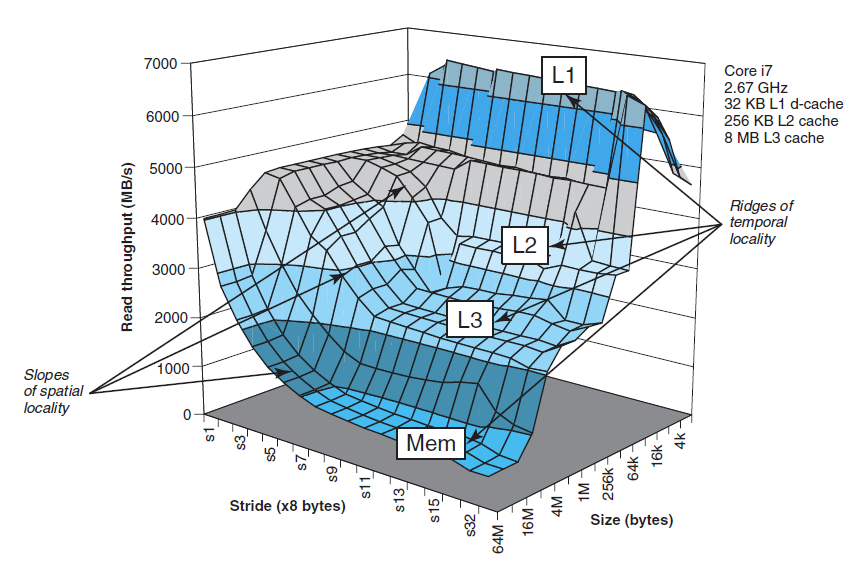
\includegraphics[width=\textwidth, height=0.5\textwidth]{PICs/memory_mountain}
	\caption{Relation of a record's stride and size to the read throughput, characterized as the memory mountain. \mcppic{bryant}{623}}\label{memory_mountain}
\end{figure}
Even a split that divides contextual relation might result in a performance boost, if only the cold data is 'cold enough', but just as well a bad split might result in even worse cache utilization.
In order to make a decision, that regards temporal- and spatial locality in a complex situation, we might need to find a way to evaluate, compare and eventually prioritize individual fields. An attempt to solve this will be made in the prototypical implementation, so more on that later on in \refsec{prototype}.

\subsubsection{Components}
After a grouping procedure the remnant members of the original NPC class could also be grouped by the same method that was mentioned before: take related members unify them in a struct and store those structs in an array in order to create spatial locality for domain related data. If the original class hierarchy was designed well in terms of cohesion metrics, the grouping of related data bits will start to resemble it, which might look like a step backwards at first, but remember, the related data groups are packed in seperate single purpose arrays and what counts is the access patterns to retrieve them. When we are done grouping all related data bits of the original NPC object, we will have recreated a so called \textit{component pattern} \mcp{nystrom}{213}.\\
In the classical component pattern we will keep a container object that holds instances of each component \mcp{nystrom}{214}. In favor of performance the container object should only hold pointers to the instances lying in their respective array. But actually and if we were able to group all members of the original class, the object might be nothing else but an index, that can be used to retrieve a group out of its array.\\
Components are one widely used mechanism to decouple parts of a formerly shared entity. This is applied to classes and is therefore a statement to how OOP and DoD can work hand in hand. Not only is the component pattern useful for decoupling and performance interests, it also solves issues, that would normally be solved by applying multiple inheritance \mcp{nystrom}{215}, which is a practice often despised even by OOP enthusiasts.\\
Components can be stored domain wise, while still being contextually linked individually on an object instance level. Their decoupling mechanism has proven great maintainability and even provides a comparably light weight interface for game designers. Accessing them can be done domain wise as well -> optimal cache utilization. This elegant arrangement between OOP and DoD makes it a favored pattern for modern game engines \mcp{fabian}{83}.
\subsubsection{Array Of Structure Of Arrays (AOSOA)}\label{aosoa}
\begin{wrapfigure}[9]{r}{0.4\textwidth}
\vspace{-1.4cm}
\begin{lstlisting}[language=C++,numbers=none,name={AOSOA variant of grouped NPC traits},label={aosoa_npc}]
struct npc_bucket{
	float
	xyz[3] [SUB_SET_SIZE],
	vel[3] [SUB_SET_SIZE],
	mass   [SUB_SET_SIZE],
	damping[SUB_SET_SIZE];
};

npc_bucket npc_buckets[NUM_BUCKETS];
\end{lstlisting}
\end{wrapfigure}
At first glance the idea of reintroducing the AOS concept seems confusing. In some cases depending on the original access patterns it might however be a good idea to separate the total amount of data into chunks that are often referred to as \textit{Buckets} or \textit{Tiles}. We already went a step back before, when we decided to unify logically related bits and make arrays of groups. We figured, that this might be an optimal solution for a very specific computation, but might behave poorly in other situations. Whenever data is grouped we might have the same problem, we tried to get rid of in the first place - possibly loading unwanted data into the cache, increasing access latency. The moment we decide, that for example our game should play a scary sound when the players distance to an NPC falls below a certain threshold, we again would be doomed to load adherent information about the NPC's velocity, mass and stuff that was grouped to make position updates faster. Because for this we actually only want the NPCs' positions.\\
An attempt to solve this, is to yet again separate the relevant members, however to a certain extend gain back the advantage of spatial locality. Applied to our NPC it might look like \refcode{aosoa_npc}. We merely define our former \textit{columns}/arrays to hold only a subset of the total data respectively. The structures, that hold our member-arrays (the SOA) will however now be emplaced inside an array itself (the AO)! In Other words: We keep the data that will be used to transform each other close to prevent eviction. We enable the user to access specific subsets individually, to prevent/appease loading unnecessary information. \textit{The idea here is to get the benefit of locality at the outer-level and also unit-stride at the innermost-level} \mc{aosoa}. This attempt is compossible with grouping certain members, too. After all we are still able to access only specific sub arrays of buckets. A bucket should consist of logically related data, so we know that for a bucket's member array $a_{n}$ and an element index $npc_{e}$ each member array $a_{0\dotsc n-1}$ of a bucket contains data that is relevant to a distinct set of computations at position $npc_{e}$. For example $npc\_buckets[0].xyz[1]$ and $npc\_buckets[0].vel[1]$ will contribute to a distinct computation since they are used to describe a single abstract entity's state.\\
Finding the NPC nearest to the player would now mean iterating the \textit{xyz} subsets of each bucket. Depending on the data bundled in a bucket (especially concerning alignment and padding) we still need to expect to load unwanted data subsequently to \textit{xyz} but this will now happen on a \textit{per-bucket} basis rather than on a \textit{per-NPC} basis.\\\\
A crucial factor to the performance of an AOSOA data layout is its subset size and the resulting \textit{bucket-size\textbf{:}number-buckets} ratio. In case of our \refcode{aosoa_npc} example, taken to the extreme $\textit{NUM\_BUCKETS}=1$ would practically result in the classic SOA model, coming with all its advantages and disadvantages. On the other hand $\textit{SUB\_SET\_SIZE}=1$ would pretty much just be an object definition again (so AOS only needlessly more confusing and incomplete since we may have grouped the members).\\
Concerning our \textit{SUB\_SET\_SIZE}, independent of a cache's associativity, the \textit{eviction} of elements inside contiguous blocks of memory  will only ever occur when the data's size exceeds the cache's capacity (not considering other processes). One first conclusion could be, that our bucket's size should not exceed our L1 D cache capacity (e.g. 32KiB), to guarantee, that the adressable unit at $a_n + npc_e$ will not be evicted by access on $a_{n+1}+npc_e$ nor by any access on $a_t+npc_e$ where $t > n$.\\
Additionally \mcp{intel}{61} advises us to "\textit{Optimize data structures [...] to fit in one-half of the first-level cache [...]}" (e.g. 16KiB) because the cache is hardware and therefore shared by all processes currently running. We usually ca not expect exclusive access and full cache capacity exploitation. Demanding all resources might perform well in a situation where no other processes demand frequent main memory access. It might also be prone to eviction when the systems workload is increased. Multi way associativity techniques accommodate us to great amounts in this case, but the moment we are trying to utilize a cache in its entirety we foster concurrency between processes, that will eventually affect the entire system.\\
Going even further \mcp{intel}{3;66} warns about it's L2 hardware prefetching mechanisms to only work within page boundaries (e.g. 4KiB), so making sure a bucket fits this criteria we could further advance optimal prefetching behavior, because we ensure, that no $a_n+npc_e$ and $a_n+npc_{e+1}$ will exceed a page boundary. This complies to the principle of page locality \mc{aosoa}.\\
We're not even done yet. AOSOA  perfectly suffices parallelization. Dependent, on which cache level is shared among the CPUs/Cores we could further optimize against it by adapting our bucket's size to for example an L2 128 Byte cache-line, resulting in a \textit{SUB\_SET\_SIZE} of $\frac{128}{8\times sizeof(float)} = 4$, guaranteeing minimal cache-level synchronization overhead.\\
Another approach could be to determine the ratio between \textit{single-entity-access-patterns} to \textit{domain-related-access-patterns} in the source program. The more our application relies on entity-access patterns, meaning we want all or most of an entity's members (classic OOP access) the smaller our subsets could be. On the other hand, the more our application relies on domain-related access patterns, meaning we want one or a few of our entities' specific members, the greater our subsets should be.\\\\
The AOSOA pattern is highly flexible making it a fit for a lot of use cases. Its limitations are defined by the minimal bucket size and the optimization goals. The Buckets' sizes can be modified at compile time or at run time. This way even when one ca not reason about subset sizes, there is still the possibility to just try out different iterations and document changes in performance/cache utilization.


\chapter{Motivation}\label{motivation}
We have now seen some of the fundamental differences between \textit{Object Oriented Programming} and \textit{Data oriented Design}. After recognizing the existence of a \textit{memory gap} we got to know some of the memory units our modern computer architectures are composed of. This helped us understanding why the caching technologies we make use of today tolerate but do not thrive on the real world metaphors we use to design our data models.\\
We learned that DoD offers methods that comply to our modern hardware, by trading abstraction as well as readability in exchange for performance. So in terms of utilizing the memory hierarchy it is inarguable superior to OOP. But we have also identified abstraction as one of the most important concepts in programming \mcp{bryant}{24} and to be one of the most important skills a programmer can have, since it is directly linked to a humans capability to solve a problem. We came to an understanding, that the abstraction model, that OOP inherits to us is widely accepted and applied in the industry, because it is intuitive and easy to learn.\\
Even when one is ready to abandon OOP it will persist. The industry is known for its reluctance to change. Implementing a new programming language into a developer team might be beneficial in long term, but comes with less to zero temporary productivity and initial training. Also DoD requires an understanding of hardware concerns, that novices and fresh graduates might not have. Most projects and companies are not even that dependent on high performance code, instead rely on solutions, that are quickly developed and easy to maintain and for the same reasons even the games industry won't solely rely on DoD probably ever. We also depend on gameplay programmers or level designers who will interact with an engine heavily but should not have to think about the underlying hardware all the time \mcp{fabian}{260}. The point is: No matter how much better other programming paradigms are on certain viewpoints and for specific tasks, OOP has its \textit{raison d'etre}. Instead of trying to sort it out we might just try to find a way to get the best out of both worlds.

\subsubsection{The best out of both worlds}
We already determined that DoD and OOP can get along to certain extends \refsecp{rtasl}. The more we want to rely on DoD to obtain performance boosts however, the more we will dismantle our abstraction step by step. Ideally we could keep whats best about OOP and still have optimal performance as though we had implemented our idea using DoD.\\
As mentioned before in \refsec{oop_bad_abstraction} DoD is not inferior to OOP in terms of maintainability per se. DoD's greatest disadvantage is, that it doesn't allow us to transfer a problem into code, the way we perceive it in the real world. The intuitive and thus advantageous abstraction model that comes with OOP is lost. On the other hand better performance makes a strong case for DoD, especially for game developers.\\
In conclusion what we want is the real world metaphors coming with OOP as well as the performance benefits coming from a data layout, that facilitates optimal cache utilization. Still, the question on how it is possible to achieve both things, remains.

\subsection{Native language support for DoD principles / ISPC / JAI}\label{nat_lan_sup}
There are languages in existence and under development, that aim to provide native support for SOA/AOSOA data structures!

\subsubsection{Intel's ISPC}
\begin{wrapfigure}[11]{r}{0.34\textwidth}
\vspace{-0.8cm}
\begin{lstlisting}[language=C++,name={ISPC's native SOA support},morekeywords={soa}, label={ispc_npc}]
struct npc_group{
	float x, y, z;
	float v_x, v_y, v_z;
};

soa<128> npc_group pos_and_vel;
soa<16> npc_group aosoa_pos_and_vel[8];
\end{lstlisting}
\end{wrapfigure}
The \textit{Intel SPMD Program Compiler} (ISPC) is specifically designed to support quick and easy development of \textit{Single Program Multiple Data} \textit{SPMD} applications, making use of implicit \textit{Single Instruction Multiple Data} (SIMD) vector units \mc{ispc}.\\
Those instructions depend on SOA data layouts, thus the language provides a \textit{soa} keyword to automatically transform an AOS defined struct into a SOA format. In \refcode{ispc_npc} an AOS \textit{npc\_group} is defined in line 1. In line 6 the \textit{pos\_and\_vel} is defined as a SOA holding 128 consecutive \textit{x}, \textit{y}, \textit{z}, \textit{v\_x}, \textit{v\_y}, and \textit{v\_z} respectively. This also easily enables for AOSOA format as can be seen in line 7.

\subsubsection{Jonathan Blow and JAI}
\begin{wrapfigure}[6]{r}{0.34\textwidth}
\vspace{-0.8cm}
\begin{lstlisting}[language=C++,name={JAI's native SOA support},morekeywords={SOA}, label={jai_npc}]
npc_group :: struct SOA{
	xyz : [3] float;
	vel : [3] float;
};
\end{lstlisting}
\end{wrapfigure}
A prominent game developer and critic of the C++ language Jonathan Blow for example is working on the \textit{JAI} programming language. There is currently no official documentation to it and it is unknown when the language will be released to public, but some of its features and its design goals are already well known. One of the highly anticipated features is automatic AOS to SOA conversion done by the compiler using nothing but a single keyword. There is no official documentation and information presented here originates only from the various online video talks Blow provides occasionally (e.g. \textit{Making Programming less terrible} by Jonathan Blow from 2017 \mc{jonblowtalk}). In \mc{jonblow} the \textit{SOA} keyword is introduced as a typespecifier when creating a struct, automatically informing the compiler to store the struct's members in a SOA fashion and granting correct access to them \refcodep{jai_npc}.

\subsection{High level abstraction hiding DoD}
However we already know, that introducing new languages/technologies into a functioning industry is mostly viewed as a cost factor and since C++ is the most prominent language in the game development industry, we can not expect to see a lot of native language support for DoD principles like SOA in the near future (unless the ISO C++ committee decides in its favor).\\
One possible solution could be to provide high level abstraction containers, that internally work with data oriented concepts. In his online blog article \textit{Implementing a semi-automatic structure-of-arrays data container} \mc{reinalter} Stefan Reinalter introduces a possible implementation for such mechanisms. Template meta programming is a way of interacting with the compiler and can to a certain extend overcome the inherent conflict between OOP and DoD, but Reinalter states that:
\begin{quote}
	\textit{I really would like to have a fully automatic implementation, but I don’t believe that’s possible without compiler support.} \mc{reinalter}
\end{quote}
Even when we can provide high level data containers, that implement a cache friendly data layout, it can not completely decouple the process of modeling the reality into code from reflecting about its data layout considering optimal hardware utilization. The high level containers in the end still need to be used correctly and based on implementation may require to define the relevant records dependent on it (for example with macros), because due to missing \textit{reflection} features, we can't iterate a record's members.\\
If possible an ideal solution would be uncorrupted high abstraction code, that somehow translates to high performance code. The relevant keyword here is \textit{translate}. Compilers normally do these kinds of tasks. The question arises whether we could utilize compiler technology to accomplish our goal.
\chapter{Compiler technology as a mediator between OOP and DoD}
The inherent purpose of a compiler is to read a program defined in a \textit{source language} and translate it to an equivalent pendant for a \textit{target language} \mcp{aho}{1}.\\
Compilers provide some of the most important features a programmer needs, like syntactic and semantic analysis steps, which can automate the process of finding errors and even just smelly code. To do that they need some sort of 'understanding' for the program.

\section{A compiler's understanding of the program}\label{compilers_understanding}
\begin{wrapfigure}[8]{r}{0.4\textwidth}
\vspace{-0.8cm}
	\begin{lstlisting}[numbers=none, name={Exerpt of example context free grammar defining a (if)statement. Bold = terminal; italic = nonterminal}, emph={stmt, optexpr}, emphstyle=\itshape, morekeywords={expr, if}, mathescape=true, literate={->}{$\rightarrow{}$}{1}, label={bnf}]
	stmt -> expr ;
		| if ( expr ) stmt
	\end{lstlisting}
\end{wrapfigure}
Modern compilers implement several \textit{phases} bundled in \textit{passes} to provide an abstraction rich routine from reading mere character sequences until generating char sequences in the target language \reffigp{compiler_phases}. Of course compilers are not thinking entities, but there are mechanisms to formally define a language as well as steps to generate semantic statements with it, ordering them in a way so that a computer can process them in a meaningful way.
\subsubsection{Syntax definition}
\begin{wrapfigure}[10]{l}{0.32\textwidth}
	\begin{center}
		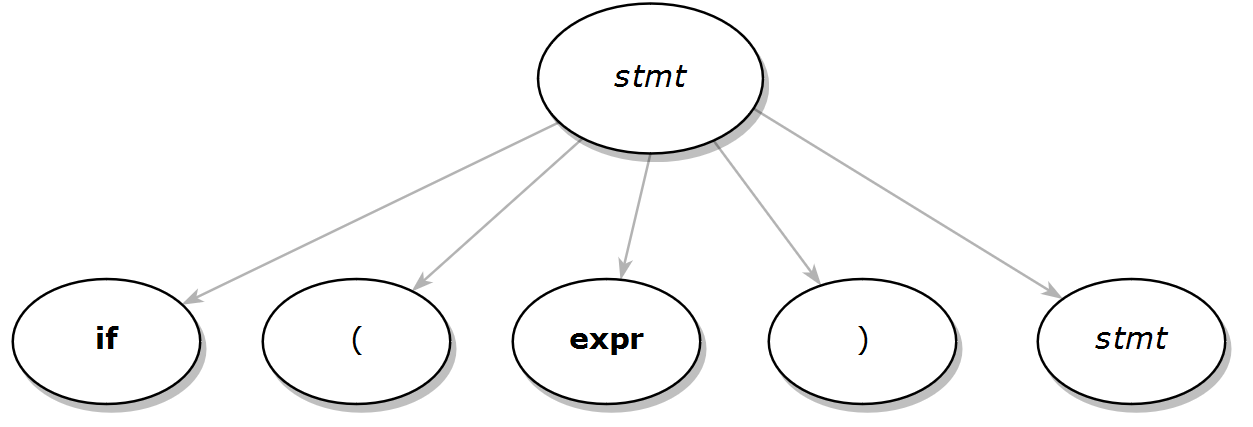
\includegraphics[width=.32\textwidth, height=0.12\textheight]{PICs/parse_tree}
	\end{center}
	\caption{Parse tree for the if-stmt node.}\label{parse_tree}
\end{wrapfigure}
\vspace{-0.5cm}
A syntactical language definition can be done using the \textit{context free grammar} notation or \textit{BNF} (Backus-Naur Form) \mcp{aho}{40}. Those grammars define a hierarchy of rules on how to form statements/expressions in the language. By defining a set of elementary symbols (\textit{terminals}) for example keywords we can then define more complex \textit{nonterminals}, like defining how a statement is formed. Ultimately we can make \textit{production} rules that describe for example our control flow statements \refcodep{bnf}. Just like this set of grammar rules basically constitutes a hierarchy, we can deduce a \textit{parse tree} for it as a concrete implementation, where beginning from the start symbol are able to derive valid successors for each symbol by iterating its child nodes. Given a statement like: "$\textit{\textbf{if} \textbf{true}) i++;}$". After reading the first token \textit{if} we can iterate our parse tree's production node for that statement and easily see, that the rule demands an opening bracket immediately following the if terminal, rendering the input as syntactically ill-formed \reffigp{parse_tree}. To be able to analyze a program like this we initially need to pass through a few \textit{phases} transforming and collecting data until we have a representation, we can work with.

\subsubsection{Lexical analysis}
\begin{wrapfigure}[20]{r}{0.2\textwidth}
\vspace{-1cm}
	\begin{center}
		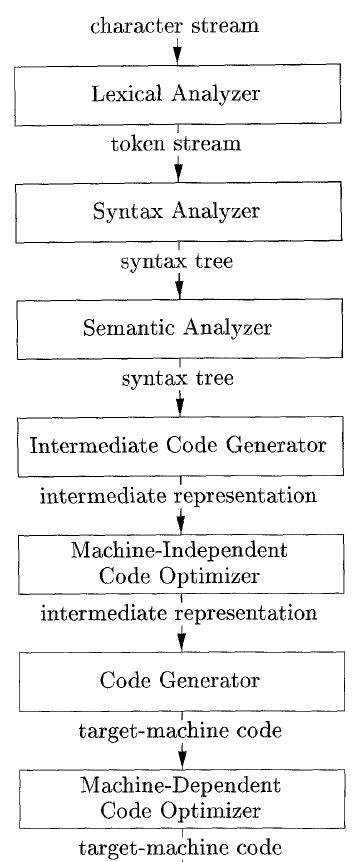
\includegraphics[width=.3\textwidth, height=0.45\textheight]{PICs/compiler_phases}
	\end{center}
	\caption{Phases of a compiler \mcppic{aho}{5}.}\label{compiler_phases}
\end{wrapfigure}
The compilers \textit{Lexer} or \textit{Scanner} takes the raw sequence of chars forming the source code and creates tokens out of char subsets it identifies as such. This information is used to fill the \textit{Symbol table}, which holds information like types, relative positions of the values, scopes and more. The symbol table is used in several following phases and essential for correct linkage of different compilation units.
\subsubsection{Syntax analysis}
The syntax analyzer creates the first \textit{Intermediate Representation} of the source code, the \textit{Syntax Tree} or \textit{Abstract Syntax Tree} (AST). It takes the token stream provided by the first phase and orders them in a tree like structure that already accounts for computational order and depicts the the grammar of the input.
\subsubsection{Semantic analysis}
Analyzing the AST from the previous phase is the \textit{Semantic Analyzer}'s duty. It traverses the AST and constantly compares its nodes with the formal language definition and gathers information like type traits. Consequently \textit{type checking} - which is important for statically typed languages - will take place in this phase \mcp{aho}{5-9}.

\section{A useful interface / LibTooling}\label{a_usfl_int}
As can be seen in \reffig{compiler_phases} there are several more phases left to describe, however \refsec{compilers_understanding} already provides information that we can utilize towards implementing a tool, that automatically translates OOP code into a cache friendly pendant.\\
Assuming we have access to our programs AST, we could start analyzing the code in an environment, that allows us to traverse the code in a tree like fashion. This means easy access to the defined data layout, as well as the access patterns in use.\\
Luckily modern compilers are designed in a modular fashion and usually define \textit{front ends} and \textit{back ends} to facilitate a multiple language to machine mapping. The front end consists of the analysis phases as well as the intermediate code generation phases for a source language. After generating an intermediate representation (IR) it is forwarded to the back end which \textit{synthesizes} the end product in the desired target language \mcp{aho}{4}.\\
The front end is especially interesting to us since it provides us with the appropriate representations to thoroughly investigate a program.

\subsubsection{LLVM/Clang}
\begin{wrapfigure}[9]{r}{0.3\textwidth}
\vspace{-20pt}
\begin{lstlisting}[language=C++,name={Example code in a Foo.cpp file},label={foo_code}]
struct Foo {
	int bar;
};

int main(){
	Foo f;
	f.bar = 10;
}
\end{lstlisting}
\end{wrapfigure}
A rather prominent representative of such an assembler/compiler/debugger tool-chain is the open source LLVM project. The front end functionality for C++ is here implemented in the Clang compiler. All the functionality is accessible and furthermore served through diverse production-grade reusable libraries and interfaces \mc{lattner} - for example the \textit{LibTooling} library that brings functionality for parsing code, creating ASTs and running \textit{FrontEndActions} over it. There are already mechanisms for recursive AST traversal like \textit{Recursive AST Visitors} and AST matching functionality with the \textit{AST Matchers}. Also tools like \textit{clang-query} provide a \textit{REPL} (Read-Eval-Print Loop) environment for quick testing.\\
In \refsec{nat_lan_sup} we saw, that languages supporting DoD natively rely on particular keywords to tag a record as SOA layouts for the compiler. We will try to carefully select the right ones using appropriate metrics (Not each record will qualify for our optimization). In case of finding any records at all it is easy enough, thanks to the functionality coming with Clang.
\begin{figure}[!htbp]
	\centering
	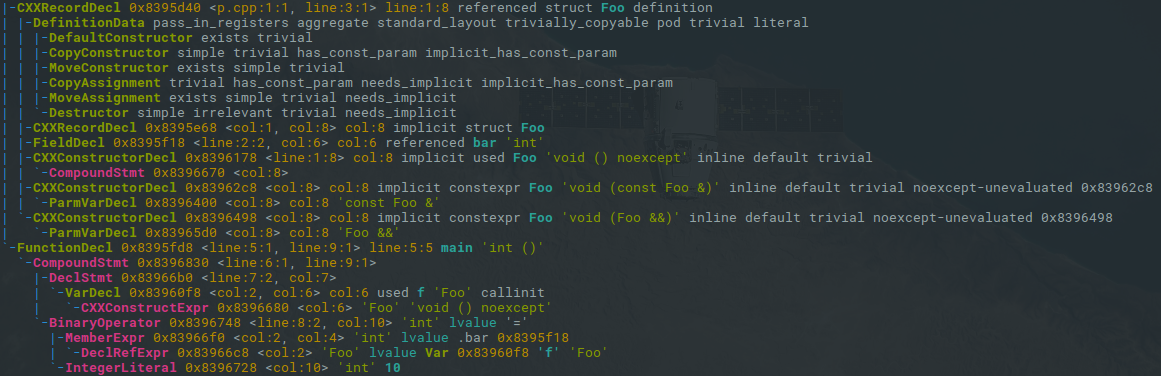
\includegraphics[width=\linewidth, height=0.5\textwidth]{PICs/foo_code_ast_dump}
	\caption{AST dump of \refcode{foo_code} generated with \textit{clang -Xclang -ast-dump Foo.cpp}.}\label{foo_code_ast_dump}
\end{figure}
The \textit{AST Matchers} and the online \textit{AST Matcher Reference} offer an excellent modular way of matching AST nodes against predefined patterns. Working with an AST is of course a lot more comfortable than working on plain text, but it also entails a new domain that one needs to familiarize with. Clang also provides proper functionality to do so. For example seeing what kind of AST nodes there are in a certain source code. When using \textit{'clang -Xclang -ast-dump Foo.cpp'} on \refcode{foo_code} among additional meta information we will see something like \reffig{foo_code_ast_dump}.
\vspace{-0.9cm}
\subsubsection{}
\begin{wrapfigure}[23]{l}{0.5\linewidth}
	\centering
	\vspace{-20pt}
	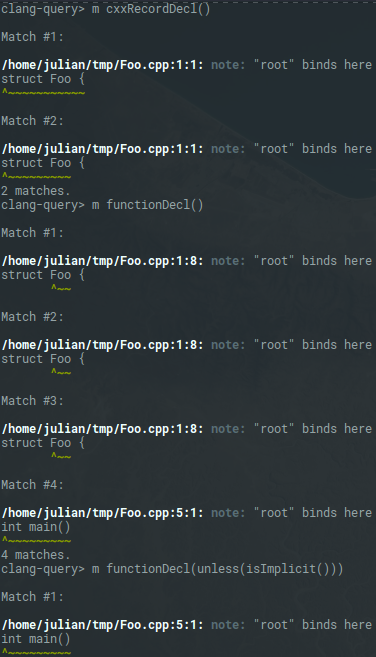
\includegraphics[width=\linewidth, height=0.7\textwidth]{PICs/clang_query_foo_code}
	\caption{AST dump of \refcode{foo_code} generated with some simple AST matchers in the easy to use \textit{clang-query} environment.}\label{foo_code_clang_query}
\end{wrapfigure}In this textual representation of the AST we can see what AST nodes make up our record (\textit{CXXRecordDecl, FieldDecl,} implicit \textit{CXXConstructorDecl}s) and how it is used (\textit{CXXConstructExpr, DeclRefExpr}). The \textit{clang-query} tool \refsecp{a_usfl_int} offers a platform for immediate testing, without setting up the rather complex structure a clang tool requires.\\
In \reffig{foo_code_clang_query} we explore some simple AST matchers like \textit{cxxRecordDecl} and \textit{functionDecl()}. Even though \refcode{foo_code} only defines one function (main) with the matcher \textit{functionDecl()} we have 4 matches. Also we do not even just match the main function but also our record's definition! This is due to implicit statements being handled the same way for matchers with low complexity. When looking up the AST matcher in the online AST Matcher Reference we will find the following documentation:\newline
\begin{lstlisting}[numbers=none, frame=none, name={AST Matcher Reference documentation for the matcher functionDecl()}]
Matcher<Decl>	functionDecl	Matcher<FunctionDecl>...

Matches function declarations.

Example matches f
void f();
\end{lstlisting}
In this case, when one is confronted with a problem the documentation does not explain, the '\textit{cfe-dev -- Clang Front End for LLVM Developers' Mailing List}' is the platform to receive help from active developers. The AST dumping mechanisms, the AST Matcher Reference, the clang-query environment and the clang mailing list as a last resort will be our sharpest swords in development.







\chapter{Quotes}
\section{hennessy}
\subsection{principle of locality}
\textit{The	most important program property that we regularly exploit is the principle of
	locality: Programs tend to reuse data and instructions they have used recently. A
	widely held rule of thumb is that a program spends 90\% of its execution time in
	only 10\% of the code. An implication of locality is that we can predict with reasonable
	accuracy what instructions and data a program will use in the near future
	based on its accesses in the recent past. The principle of locality also applies to
	data accesses, though not as strongly as to code accesses.
	Two different types of locality have been observed. Temporal locality states
	that recently accessed items are likely to be accessed in the near future. Spatial
	locality says that items whose addresses are near one another tend to be referenced
	close together in time.}
\mcp{hennessy}{38}


\section{drepper}
\subsection{cache layout}


\subsection{Lc Ld}
\textit{Even though most computers for the last several decades
	have used the von Neumann architecture, experience has
	shown that it is of advantage to separate the caches used
	for code and for data}
\mcp{Drepper}{14}


%
% Hier beginnen die Verzeichnisse.
%
\clearpage
\ifthenelse{\equal{\FHTWCitationType}{HARVARD}}{}{\bibliographystyle{gerabbrv}}
\bibliography{Literatur}
\clearpage

% Das Abbildungsverzeichnis
\listoffigures
\clearpage

% Das Tabellenverzeichnis
\listoftables
\clearpage

% Das Quellcodeverzeichnis
\listofcode
\clearpage

\phantomsection
\addcontentsline{toc}{chapter}{\listacroname}
\chapter*{\listacroname}
\begin{acronym}[XXXXX]
    \acro{ABC}[ABC]{Alphabet}
    \acro{WWW}[WWW]{world wide web}
    \acro{ROFL}[ROFL]{Rolling on floor laughing}
\end{acronym}

%
% Hier beginnt der Anhang.
%
\clearpage
\appendix
\chapter{Anhang A}
\clearpage
\chapter{Anhang B}
\end{document}